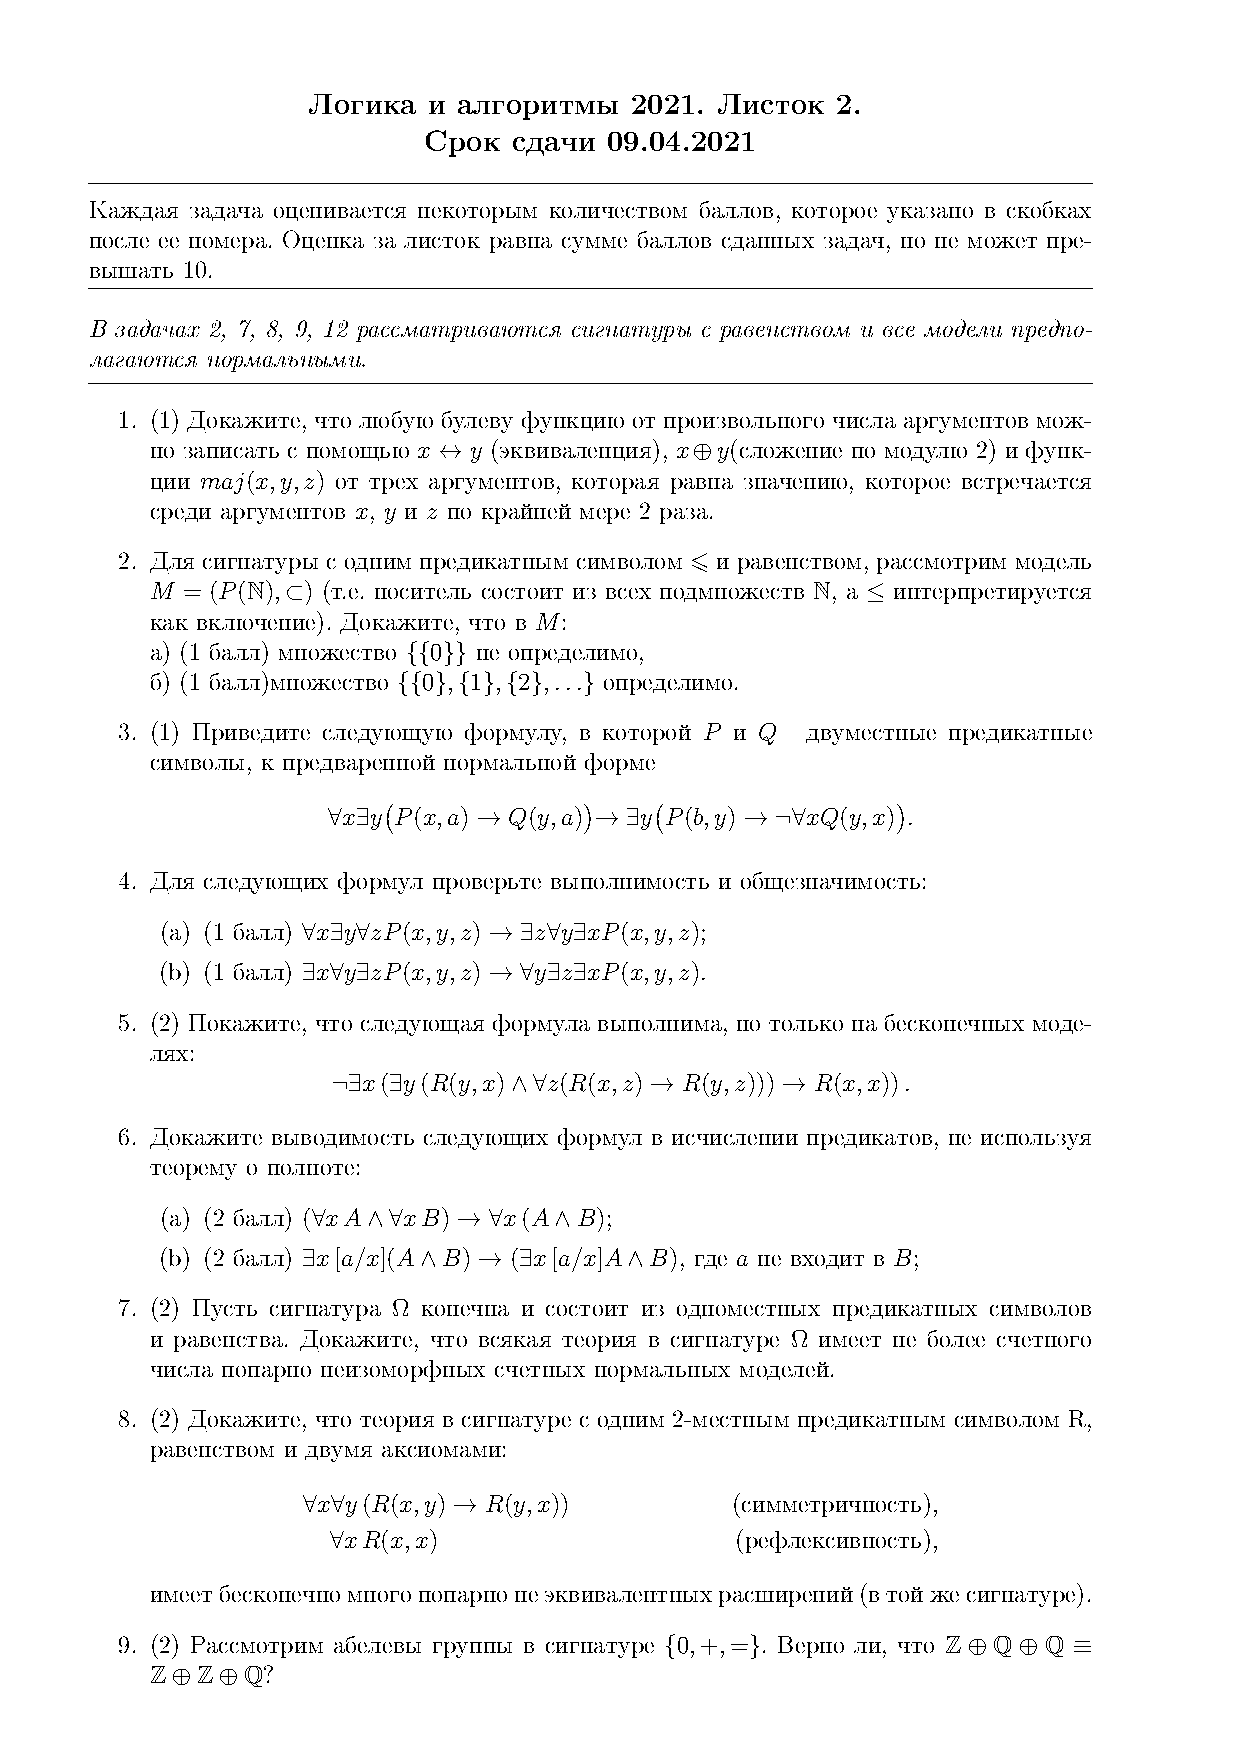
\includepdf[scale=1,pages=1-2]{Tasks/listok2}
\newpage
\section*{Решения}
\subsection*{Задача 1}
	Теорема о функциональной полноте. Для любой функции $\varphi: \mathbb{B}^n \to \mathbb{B}$ найдется такая формула $A$ от $n$ переменных, что $\varphi = \varphi_{A}$. При этом можно считать, что $A$ содержит лишь связки $\neg$ и $\vee$.\\
	Следовательно если выразить $\neg$ и $\vee$ через $x \leftrightarrow y,\ x \oplus y,\ \operatorname{maj}(x,y,z)$\\
	\begin{gather*}
	\begin{tabular}{ c c c c c c }
		x & y & x \leftrightarrow y & x \oplus y & \operatorname{maj}(x, y, x \oplus y) & x \oplus (x \leftrightarrow x)\\
		0 & 0 & 1 & 0 & 0 & 1\\
		0 & 1 & 0 & 1 & 1 & 1\\
		1 & 0 & 0 & 1 & 1 & 0\\
		1 & 1 & 1 & 0 & 1 & 0
	\end{tabular}
	\end{gather*}
	Заметим, что $\operatorname{maj}(x, y, x \oplus y)$ соответствует $x \vee y$, а $x \oplus (x \leftrightarrow x) = x \oplus 1$ соответствует $\neg x$, а следовательно любую булеву функцию можно записать, используя только данные по условию функции.

\subsection*{Задача 2}
\begin{enumerate}
\item[(a)] Рассмотрим отображение, такое что $\{0\} \leftrightarrow \{1\}$. Покажем, что это автоморфизм, то есть что если $A \subseteq B$, то $A' \subseteq B'$. Пусть $a \in A'$
	\begin{gather*}
		a \ne 0,1 \Rightarrow a \in A \Rightarrow a \in B \Rightarrow a \in B'\\
		a = 0 \Rightarrow 1 \in A \Rightarrow 1 \in B \Rightarrow 0 \in B'\\
		a = 1 \Rightarrow 0 \in A \Rightarrow 0 \in B \Rightarrow 1 \in B'
	\end{gather*}
	Итак, множество $\{\{0\}\}$ не сохранилось при рассмотренном автоморфизме, а определимые множество сохраняются при любом автоморфизме, а следовательно $\{\{0\}\}$ не явояется определимым.

\item[(b)]
	Зададим предикат, выражающий свойство одноэлементности множества, то есть всякое подмножество данного множества или пусто, или совпадает с ним самим. Выразим свойство пустоты множества ($x = \{\}$) формулой $\forall y\ x \leqslant y$, а также свойство равенства двух подмножеств ($x = y$) формулой $(x \leqslant y) \wedge (y \leqslant x)$. Через это мы можем выразить свойство одноэлементности $\forall y ((y \leqslant x) \to ((y = \{\}) \vee (y = x)))$.
\end{enumerate}
\vskip 0.4in

\subsection*{Задача 3}
	\begin{gather*}
		\forall x \exists y(P(x,a) \to Q(y,a)) \to \exists y(P(b,y) \to \neg \forall x Q(y,x))\\
		\forall x \exists y(P(x,a) \to Q(y,a)) \to \exists z(P(b,z) \to \neg \forall t Q(z,t))\\
		\forall x \exists y(\neg P(x,a) \vee Q(y,a)) \to \exists z(\neg P(b,z) \vee \neg \forall t Q(z,t))\\
		\neg \forall x \exists y(\neg P(x,a) \vee Q(y,a)) \vee \exists z(\neg P(b,z) \vee \neg \forall t Q(z,t))\\
		\neg \forall x \exists y(\neg P(x,a) \vee Q(y,a)) \vee \exists z(\neg P(b,z) \vee \exists t \neg Q(z,t))\\
		\exists x \forall y \neg (\neg P(x,a) \vee Q(y,a)) \vee \exists z(\neg P(b,z) \vee \exists t \neg Q(z,t))\\
		\exists x \forall y \exists z \exists t \neg (\neg P(x,a) \vee Q(y,a)) \vee (\neg P(b,z) \vee \neg Q(z,t))\\
		\exists x \forall y \exists z \exists t (P(x,a) \wedge \neg Q(y,a)) \vee (\neg P(b,z) \vee \neg Q(z,t))\\
		\exists x \forall y \exists z \exists t (P(x,a) \vee \neg P(b,z) \vee \neg Q(z,t)) \wedge (\neg Q(y,a) \vee \neg P(b,z) \vee \neg Q(z,t))\\
	\end{gather*}
\vskip 0.4in

\subsection*{Задача 4}
\begin{enumerate}
\item[(a)]
	\begin{gather*}
		\forall x \exists y \forall z P(x,y,z) \to \exists z \forall y \exists x P(x,y,z)
	\end{gather*}
	Рассмотрим модель целых чисел, в которой $P(x,y,z):\ y = x^2$. Тогда $\forall x \exists y \forall z (y = x^2)$ верно, а $\exists z \forall y \exists x (y = x^2)$ неверно, следовательно формула необщезначима.
\item[(b)]
	\begin{gather*}
		\exists x \forall y \exists z P(x,y,z) \to \forall y \exists z \exists x P(x,y,z)
	\end{gather*}
	Если левая часть -- истина, то существуют такие $x_0, z_0$, что $\forall y:\ P(x,y,z) \equiv 1$, тогда правая часть также истина, так как для этой же пары $x_0, z_0$ все будет выполнено, а следовательно формула истина. Если левая часть ложна, то следствие может быть любым, а следовательно формула также истина. Тогда она всегда истина, а следовательно выполнима и общезначима
\end{enumerate}
\vskip 0.4in

\subsection*{Задача 5}
	\begin{gather*}
		\neg \exists x(\exists y(R(y,x) \wedge \forall z(R(x,z) \to R(y,z))) \to R(x,x))\\
		\forall x \neg (\exists y(R(y,x) \wedge \forall z(R(x,z) \to R(y,z))) \to R(x,x))\\
		\forall x \neg (\exists y(R(y,x) \wedge \forall z(\neg R(x,z) \vee R(y,z))) \to R(x,x))\\
		\forall x \neg ( \neg \exists y(R(y,x) \wedge \forall z(\neg R(x,z) \vee R(y,z))) \vee R(x,x))\\
		\forall x (\exists y(R(y,x) \wedge \forall z(\neg R(x,z) \vee R(y,z))) \wedge \neg R(x,x))\\
		\forall x \neg R(x,x) \wedge \forall x \exists y (R(y,x) \wedge \forall z (\neg R(x,z) \vee R(y,z)))\\
		\forall x \neg R(x,x) \wedge \forall x \exists y \forall z (R(y,x) \wedge (\neg R(x,z) \vee R(y,z)))\\
		\forall x \exists y \forall z (\neg R(x,x) \wedge R(y,x) \wedge (\neg R(x,z) \vee R(y,z)))
	\end{gather*}

	\begin{comment}
		\forall x \neg R(x,x) \wedge \forall x \forall y \forall z (R(x,y) \wedge R(y,z) \to R(x,z)) \wedge \forall x\exists y R(x,y)\\
		\forall x \neg R(x,x) \wedge \forall x \forall y \forall z (\neg(R(x,y) \wedge R(y,z)) \vee R(x,z)) \wedge \forall x\exists y R(x,y)\\
		\forall x \neg R(x,x) \wedge \forall x \forall y \forall z (\neg R(x,y) \vee \neg R(y,z) \vee R(x,z)) \wedge \forall x\exists y R(x,y)
	Заметим что эта формула представляет из себя 2 аксиомы арифметики Пеано: $\forall x \exists y S(x) = y$ что то же самое что $\forall x \exists y R(x,y)$ и $\forall x \forall y S(x) = S(y) \to x = y$, что то же самое что $\forall x \forall y \forall z R(y,x) \wedge (\neg R(x,z) \vee R(y,z))$, этих аксиом достаточно для того, чтобы доказать бесконечность натуральных чисел, а следовательно данная форма выполнена только для бесконечных моделей
	\end{comment}
\vskip 0.4in

\subsection*{Задача 6}
\begin{enumerate}
\item[(a)]
	Правило Бернайса $\frac{A \to B}{A \to \forall x B[a/x]}$, следовательно нам достаточно доказать, что $(\forall x A \wedge \forall x B) \to A \wedge B$ выводимо.\\
	Применим теорему о дедукции: $\Gamma \vee \{P\} \vdash Q \Leftrightarrow \Gamma \vdash P \to Q$, то есть будем выводить $A \wedge B$ из аксиом и $(\forall x\ A \wedge \forall x\ B)$\\
	Аксиомы:\\
	$A \wedge B \to A$ (1), $A \wedge B \to B$ (2), $A \to (B \to A \wedge B)$ (3)\\
	$\forall x A[a/x] \to A[a/t]$ (4), $A[a/t] \to \exists x A[a/x]$ (5)\\
	Modus ponens: $\frac{A,\ A \to B}{B}$ (MP)
	\begin{gather*}
		\forall x A \wedge \forall x B \xrightarrow{\text{(1)}}
		\forall x A \xrightarrow{\text{(4)}}
		A \xrightarrow{\text{(*)}}
		A \wedge B
		\\
		\forall x A \wedge \forall x B \xrightarrow{\text{(2)}}
		\forall x B \xrightarrow{\text{(4)}}
		B\\
		\\
		\text{(*): } (A \to (B \to A \wedge B)) \xrightarrow{\text{(MP)}}
		(A \to A \wedge B) \xrightarrow{\text{(MP)}}
		A \wedge B
	\end{gather*}
\begin{comment}
\item[(b)]
	Правило Бернсайса: $\frac{B \to A}{\exists x\ B[a/x] \to A}$, следовательно достаточно доказать, что $A \wedge B \to \exists x [a/x]A \wedge B$ выводимо.\\
	Аналогично по теореме о дедукции выведем $\exists x [a/x] A \wedge B$ из аксиом $A \wedge B$
	\begin{gather*}
		A \wedge B\\
		A \text{ -- (1)}\\
		\exists x [a/x] A \text{ -- (5)}\\
		(B \to \exists x [a/x] A \wedge B) \text{ -- (3)}\\
		\exists x [a/x] A \text{ -- (MP)}\\
		\exists x [a/x] A \wedge B \text{ -- (MP)}
	\end{gather*}
	(в (3) в качестве $A$ выступает $\exists x [a/x] A$, в качестве $B -- B$)
	и
	\begin{gather*}
		A \wedge B\\
		B \text{ -- (2)}
	\end{gather*}
\end{comment}	
\end{enumerate}
\vskip 0.4in

\subsection*{Задача 9}
	Рассмотрим формулу
	\begin{gather*}
		\forall x (\forall s\ x \ne s + s) \to (\forall y (\forall t\ y \ne t + t) \to \exists w\ x + y = w + w)
	\end{gather*}
	Пусть $\mathbb{Z} \oplus \mathbb{Q} \oplus \mathbb{Q} = M_1,\ \mathbb{Z} \oplus \mathbb{Z} \oplus \mathbb{Q} = M_2$
	\vskip 0.1in
	Эта формула всегда верна в $M_1$:\\
	Пусть $x \ne s + s\ \forall s$, это значит, что $x = (\text{нечетное}, \text{любое}, \text{любое})$, так как га второй и третьей позиции рациональные числа, там можно любое число представить в виде $\frac{\text{число}}{2}$. Пусть $y \ne t+t$, тогда аналог $y = (\text{нечетное}, \text{любое}, \text{любое})$. Тогда $x + y = (\text{нечетное}, \text{любое}, \text{любое}) + (\text{нечетное}, \text{любое}, \text{любое}) = (\text{четное}, \text{любое}, \text{любое})$, то есть формула примет вид $1 \to (1 \to 1) = 1$\\
	Если $x \ne s + s,\ y = t + t$, то $x + y = (\text{нечетное}, \text{любое}, \text{любое})$ и формула примет вид $1 \to (0 \to 0) = 1 \to 1 = 1$\\
	Если $x = s + s,\ y \ne t + t$, то $x + y = (\text{нечетное}, \text{любое}, \text{любое})$ и формула примет вид $0 \to (1 \to 0) = 0 \to 0 = 1$\\
	Если $x = s + s,\ y = t + t$, то $x + y = (\text{четное}, \text{любое}, \text{любое})$ и формула примет вид $0 \to (0 \to 1) = 0 \to 1 = 1$
	\vskip 0.1in
	Но в $M_2$ эта формула не всегда верна, рассмотрим следующий случай:\\
	$x = (1,0,0),\ y = (0,1,0),\ x + y = (1,1,0)$. Тогда формула примет вид $1 \to (1 \to 0) = 1 \to 0 = 0$, то есть они не изоморфны и утверждение задачи неверно.